% !TEX root = ../t.tex
\mktitle{通过统一交互式算法可视化网站学习算法}{Steven HALIM,Zi Chun KOH,Victor Bo Huai LOH,Felix HALIM}
% !TEX root = ../../t.tex
\mkabstract{
我们在 \url{http://www.comp.nus.edu.sg/~stevenha/visualization} 上实现了一个统一交互式算法可视化网站,其中包括各种经典或非经典的算法。相比其他许多算法可视化的网站,我们所提供的算法可视化有以下几点优势:(1)支持各种非经典算法,这些算法现在还没有在其他网站上实现过;(2)拥有交互式特性。用户(通常为学生)可以输入他们自己的数据来测试算法;(3)提供统一的用户界面;(4)使用HTML5搭建,兼容当前可携带个人电脑,包括平板和智能手机。我们在新加坡国立大学的两个算法课程班上进行用户研究,结果显示我们的可视化系统对于一些偏向于可视化学习的学生有很大的帮助。
}{
统一,交互式,算法,可视化
}

% !TEX root = ../../t.tex
\chapter{引言}
\begin{sectext}
要教授《数据结构与算法》(此后用《算法》指代)这门计算机科学中具有代表性的课程,教授、讲师、导师或者老师(此后用老师指代)都会用实际例子演示某个算法如何执行。通常的教学方法有如下几种:
\begin{itemlist}
\item 把一些静态图片或图表的例子提前打印在材料、课本或者PowerPont(或者其他类似的演示软件)的幻灯片中。如果要效果稍微好一点,就使用准备好的幻灯片动画来说明算法步骤。这种方法的缺点在于老师控制动画的速度可能会太快。另外,也很难展示其他没有嵌入的例子或者是学生当场提出的例子;老师只能直接手工画在PowerPoint的幻灯片上(用鼠标或者铁笔)或者用手在黑板上画(方法2)。

\item 老师在黑板上画出例子。不同于PowerPoint,老师不会过快跳到下一张幻灯片,这样手绘的方法让学生们能够以正常人类(学生)的节奏消化算法步骤,但画出算法的每一步可能需要一些时间。而缺点就在于这样的人工手绘太消耗时间,特别是在算法执行或准备出错的时候。同时如果算法复杂或者老师太过着急都容易出现错误。而学生们理解算法的同时,为了课后复习也会记录下老师的例子。这样一来就有冲突,学生一边需要记忆算法,另一方面有手动记录例子,如果错过了课程可能会恶化学习效果。

\item 老师只是想学生们指出可以去某些现有的算法动画网站(通常是由独立开发者创建)。其中一些网站能够有效教授算法,这些内容会在第二节中展开。但是这种方法的缺点在于大部分这些网站只题够一些经典算法的可视化。因此,如果老师对于一个算法提供一个网站,另一个算法有提供其他的网站,学生们就会因为网站不同的操作和布局感到难以理解。这些网站中各种不同的用户界面加大了学生学习的难度。一些学生可能还存在惰性现象而没有主动访问这些网站。同时,如果在教授一个少见的非经典算法时,没有网站提供可视化,那么这种方法也不可取。
\end{itemlist}

综上,教授算法更好的方法在于既能够提供带有动画的典型而且提前准备好的例子(用来初次介绍概念),又能供结合二至三个学生自己输入的例子。要使这样的方法高效需要满足两个条件:即时的例子必须在动画过程中保持结果一致而且无差错;这样的方法不能占用太多时间。
我们决定通过浏览器搭建一个基于网络的平台来实现可视化,这样全世界就有更多的人能够接触到算法知识。几乎现在所有的设备——台式电脑、笔记本,甚至是智能手机,全都带有内置浏览器,例如火狐浏览器、谷歌浏览器、苹果浏览器等等,这些都原生支持HTML5。因此无需安装任何程序,也没有跨平台的问题。

交互式而非静态可视化是因为学生对于算法可以获得更加深刻的理解。我们相信如果学生能够自己输入一些数据,那么就更加有利于理解算法的执行。

随着越来越多的可携带设备支持网络连接:笔记本、平板电脑和智能手机,许多学生可以在授课或者听讲老师的例子时用自己的设备访问我们的在线可视化网站,在课后也可以按照自己的节奏巩固算法执行过程。

在教学方面,有了这样的可视化网站,测验中许多只测试学生算法如何运行的问题也会减少。学生会更期待了解算法如何运行,所以这样的问题也变得多余起来。同时,老师也能够集中精力,出一些算法高级用法的题目。

统一的界面有利与学生学习。毫无疑问,一个典型的计算机科学课程会涉及一个算法以上。有了统一的界面,学生在使用的时候不会感到陌生。同时在整个学期中只需要将一个网页保存为书签,相比保存一大堆不同的网站更加简便。学生也不需要为了找到老师提供的网站而查阅课程的幻灯片或者材料。所有多余的不便都会对学生产生惰性,很可能导致学生偷懒,不愿理解算法含义。

这篇论文的结构如下:在第二节中,我们具体分析当前的一些算法可视化网站,算法选自''高级编程2''(Halim和Halim,2011)。这本高级编程手册有本论文的第一位作者和最后一位作者一同编写。这本书讨论了大量算法,其中许多算法都还没有可视化。同时我们还讨论了现有可视化的缺点,评判的标准是基于我们所想要达到的目标,也就是:可视化非经典算法,统一界面,交互输入用户提供的数据,兼容各设备端的浏览器,特别是智能手机。在第三节中,我们讨论了可视化系统的细节。在第四节中则汇报了来自新加坡过来立大学的31名学生最初的反馈,这些学生在2011--2012学年的第二学期使用了可视化系统的第一个版本。在第五节,就可视化系统的效果列出一些初步得到的结论,最后通过计划近期不断加强可视化系统总结全文。
\end{sectext}

% !TEX root = ../../t.tex
\chapter{现有的算法可视化网站}
\begin{sectext}
本节总结了我们对于截至2012年4月不同算法可视化网站的分析。以下的报告不考虑非在线的算法可视化。所有的算法的来自与``高级编程2''这本手册(Halim和Halim,2011)。在分析中,我们发现经典算法和非经典算法数量上的不平衡。经典算法——通常比较简单——例如排序、有序数列的二分查找等,而非经典和少见的算法——通常比较困难——例如树状数组(Fenwick,1994)、有向图的强连通分支(Tarjan,1972),网络的最大流(Edmonds和Karp,1972)等。
\end{sectext}
\section{单一可视化}
\begin{sectext}
我们把得到的记过分为两类:单一的可视化和统一可视化。表\ref{tab:1}中为单一的现有算法可视化网站,这些网站只有一到三个算法动画,开发者没有可视化其他的算法。这增加了学生的学习的负担,学生们在学习不同算法时不得不访问不同的网站。为了简化表\ref{tab:1},我们只选择了几个有代表性的经典算法可视化的网站。
% !TEX root = ../../t.tex
\begin{center}
\setstretch{1.35}
\vspace{-20pt}
\begin{longtable}{p{4cm} p{8cm} l l l}
\caption{单一可视化(截至2012年4月所有URL地址均可以访问)}
\label{tab:1} \\

\hline \multicolumn{1}{l}{主题} & \multicolumn{1}{l}{算法可视化网站地址} & \multicolumn{1}{c}{N} & \multicolumn{1}{c}{H} & \multicolumn{1}{c}{O}\\ \hline
\endfirsthead

\multicolumn{5}{r}%
{接表 \ref{tab:1}} \\
\hline \multicolumn{1}{l}{主题} & \multicolumn{1}{l}{算法可视化网站地址} & \multicolumn{1}{c}{N} & \multicolumn{1}{c}{H} & \multicolumn{1}{c}{O}\\ \hline
\endhead

\hline \multicolumn{5}{r}{待续}
\endfoot

\hline
\endlastfoot

{各种线性数据结构} & \url{apbrwww5.apsu.edu/myersb2/linked_list_animation.htm} & & H & O \\
& \url{www.u-www.cosc.canterbury.ac.nz/mukundan/dsal/StackAppl.html} & & H & O \\
{各种排序算法} & \url{www.cs.auckland.ac.nz/∼jmor159/PLDS210/Java/q_sort/tqs_new.html} & & H & O \\
& \url{www.cse.iitk.ac.in/users/dsrkg/cs210/applets/sortingII/mergeSort/mergeSort.html} & & & O \\
& \url{www.cs.oswego.edu/∼mohammad/classes/csc241/samples/sort/Sort2-E.html} & & H & O \\
位掩码或位操作 & (见4.1) & N & & \\
{基本的二叉搜索树(表格)} & \url{aleph0.clarku.edu/~achou/cs102/examples/bst_animation/BST-Example.html} & & & O \\
& \url{www.cs.jhu.edu/~goodrich/dsa/trees/btree.html} & & & O \\
& \url{www.csc.liv.ac.uk/~ullrich/COMP102/applets/bstree/} & & & O \\
{平衡树(AVL)} & \url{webdiis.unizar.es/asignaturas/EDA/AVLTree/avltree.html} & & & O \\
& \url{www.site.uottawa.ca/~stan/csi2514/applets/avl/BT.html} & & & O \\
& \url{www.cs.jhu.edu/~goodrich/dsa/trees/avltree.html} & & & O \\
{堆(优先队列)} & \url{nova.umuc.edu/~jarc/idsv/lesson2.html} & & & O \\
& \url{www.cs.auckland.ac.nz/~jmor159/PLDS210/heaps.html} & & & O \\
{图数据结构(邻接矩阵或邻接表)} & (\url{nova.umuc.edu/~jarc/idsv/} 中有一部分相关主题) & N & & \\
& (见4.4) & & & \\
{并查集} & \url{research.cs.vt.edu/AVresearch/UF/} & & & O \\
& \url{www.cs.unm.edu/~rlpm/499/uf.html} & & & O \\
Segment tree & (我们的项目今后会增加这种算法) & N & & \\
树状数组 & (见4.3) & N & & \\
{N皇后问题} & \url{www.animatedrecursion.com/advanced/the_eight_queens_problem.html} & & H & O \\
& \url{yuval.bar-or.org/index.php?item=9} & & H & O \\
经典动态规划 & (今后会增加这种算法) & N & & \\
{图的遍历:BFS/DFS等} & \url{www.cs.sunysb.edu/~skiena/combinatorica/animations/search.html} & & H & \\
& \url{www.rci.rutgers.edu/~cfs/472_html/AI_SEARCH/SearchAnimations.html} & & H & \\
割点、桥、强连通分量 & (见4.4) & N & & \\
{MST (Prim算法)} & \url{www.unf.edu/~wkloster/foundations/PrimApplet/PrimApplet.htm} & & H & O \\
& \url{students.ceid.upatras.gr/~papagel/project/prim.htm} & & H & O \\
{MST (Kruskal算法)} & \url{www.unf.edu/~wkloster/foundations/KruskalApplet/KruskalApplet.htm} & & H & O \\
& \url{students.ceid.upatras.gr/~papagel/project/kruskal.htm} & & H & O \\
SSSP (Bellman Ford算法)& (见4.7) & N & & \\
{SSSP (Dijkstra算法)} & \url{www.unf.edu/~wkloster/foundations/DijkstraApplet/DijkstraApplet.htm} & & H & O \\
& \url{www.dgp.toronto.edu/~jstewart/270/9798s/Laffra/DijkstraApplet.html} & & & O \\
APSP (弗洛伊德算法) & \url{www.pms.ifi.lmu.de/lehre/compgeometry/Gosper/shortest_path/shortest_path.html} & & H & O \\
网络流(Edmonds Karp算法) & \url{felix-halim.net/research/maxflow/index.php} & & H & O \\
&\url{www.eecs.wsu.edu/∼cook/aa/lectures/applets/ek/MaxFlowHome.html} & & H & O \\
DAG算法 & (今后会增加这种算法,包括:拓扑排序、最短/长路径、路径数) & N & & \\
树上的算法 & (今后会增加这种算法,包括:最短/长路径、所有点对最短路径、最近公共祖先) & N & & \\
二分图算法 & \url{www-b2.is.tokushima-u.ac.jp/~ikeda/suuri/main/index.shtml} & & H & O \\
字符串匹配 & \url{cgjennings.ca/fjs/index.html} & & & O \\
{后缀树} & \url{illya-keeplearning.blogspot.com/2009/06/suffix-trees-java-applet.html} & & & O \\
后缀数组 & \url{felix-halim.net/pg/suffix-array} & & & \\
多边形算法 & (见4.9) & N & & \\
% \multirow{3}{*}{\begin{minipage}{4cm}二维凸包 (Graham扫描算法,Andrew单调链算法,Jarvis卷包裹算法)\end{minipage}} & \url{www.cs.princeton.edu/courses/archive/spr10/cos226/demo/ah/GrahamScan.html} & & H & O \\
% \multirow{3}{*}{\parbox{4cm}{二维凸包 (Graham扫描算法,Andrew单调链算法,Jarvis卷包裹算法)}} & \url{www.cs.princeton.edu/courses/archive/spr10/cos226/demo/ah/GrahamScan.html} & & H & O \\
凸包 (Graham扫描、Andrew单调链、Jarvis卷包裹算法) & \url{www.cs.princeton.edu/courses/archive/spr10/cos226/demo/ah/GrahamScan.html} & & H & O \\
&\url{nms.lcs.mit.edu/ ∼ aklmiu/6.838/convexhull/} & & & O \\
&\url{www.cs.unc.edu/∼snoeyink/demos/ch/Jarvis.html} & & & O \\
\end{longtable}
\end{center}

\vspace{-5pt}

在同一个表中,我们用以下记号强调了三个可能的问题,这些问题源自我们的目标,已经在第一节中列出:
\begin{itemlist}
\item N(少见):这种算法少见,在因特网上用相关关键词搜索后没能得到可视化网站的结果。

\item H(静态,非交互式):这种算法使用内嵌的例子(包括使用动态的GIF图),用户不能通过输入新的数据来观察算法如何执行。

\item O(技术过时):这种(过时的)算法可视化使用的是以前的技术(例如Flash、Java小应用程序),不完全支持便携式设备,通过现代的智能手机(例如iPhone)或者平板电脑(例如iPad)不能访问。

\end{itemlist}

\end{sectext}
\section{统一可视化}
\begin{sectext}
除了表\ref{tab:1}中的单一可视化,我们也发现以下的统一可视化,这些可视化网站提供了三个以上的可视化:
\begin{itemlist}
\item  \url{algoviz.org} 基本上作为一个网站入口,题够不同算法可视化的网站链接。以后我们的可视化网站也将列入其中。但是,截至2012年4月,一些第三节中列出的算法可视化(例如树状数组、强连通分量等)还没有被列出。

\item  \url{www.ansatt.hig.no/frodeh/algmet/animate.html} 是另外一个网站入口,同样手机了其他可视化网站的链接。(与 \url{algoviz.org} 本质相同)

\item  \url{nova.umuc.edu/~jarc/idsv/} 提供的可视化包括:二叉树、几种图的表示和算法以及排序。

\item  \url{www.csse.monash.edu.au/~dwa/Animations/index.html} 提供的一些算法可视化与 \url{nova.umuc.edu/~jarc/idsv/} 类似。

\item  \url{research.cs.vt.edu/AVresearch/} 提供一部分算法可视化,从2003年到2009年进行维护开发。

\item  \url{www.cs.usfca.edu/~galles/visualization/Algorithms.html} 是最接近统一可视化的网站,与本论文提出的观点最为相近。同时该网站使用HTML5技术。我们会在第三节中突出我们的可视化网站与该网站的不同之处。
\end{itemlist}
\end{sectext}

% !TEX root = ../../t.tex
\chapter{统一交互式的算法可视化网站}
\begin{sectext}
这就是我们截至2012年4月所搭建的算法可视化网站。以下集中讨论的是网站初期阶段,提供的是一些非经典算法的可视化,而不是经典算法的可视化。同时我们将该网站的可视化与网上其他人编写的算法可视化比较,突出其不同之处和我们添加的额外的特点。
\end{sectext}
\section{位掩码、位操作、位串、轻量级布尔值}
\begin{sectext}
整数的位操作(位掩码)对于计算机科学的初学者相对比较微妙。因此,设计一个没有错误的位掩码可视化有助于老师展示不同例子,也有助于学生理解概念。如下面的图所示,例如,$42 | (1 << 2) = 46$。这中基于文本的可视化(如图\ref{fig:1})可以立刻显示必要的位操作。我们现在还没在网上发现其他类似可视化。
% !TEX root = ../../t.tex
\setlength{\belowcaptionskip}{-10pt}
\vspace{-7pt}
\begin{figure}[!htbp]
  \centering
  \frame{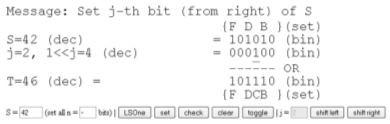
\includegraphics{img/t1}}
  \vspace{-5pt}
  \caption{位掩码的可视化}
  \label{fig:1}
\end{figure}
% \vspace{-10pt}


\end{sectext}
\section{二叉堆(优先队列)}
\begin{sectext}
二叉堆是一种经典的数据结构,通常用于实现优先队列。因特网上有许多其他类似的可视化。在这个可视化中(如图\ref{fig:2}),比起其他的可视化而言,唯一一个优点在于我们的网站拥有统一的风格。
% !TEX root = ../../t.tex
\setlength{\belowcaptionskip}{-10pt}
\vspace{-7pt}
\begin{figure}[!htbp]
  \centering
  \frame{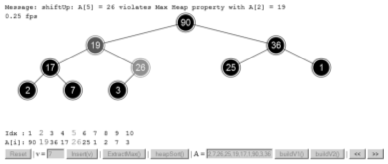
\includegraphics{img/t2}}
  \vspace{-5pt}
  \caption{二叉堆的可视化}
  \label{fig:2}
\end{figure}
% \vspace{-10pt}

\end{sectext}
\section{树状数组}
\begin{sectext}
树状数组由Fenwick(1994)发明。这种数据结构用于高效计算动态区间和查询(RSQ或者累积和频率表),由于在程序竞赛中能发挥奇特的作用,现在已经列入国际信息学奥林匹亚课程的讲解中,参加竞赛的(高中)学生都会学习。树状数组的操作对于初学者可能比较神秘。例如,$RSQ(1, 6)$是$RSQ(1, 4)+RSQ(5, 6)$的和,因为把整数6(二进制表示为``110'')最右边的1截去就变成了4(二进制表示为``100''),再做一次,整数4就变成了0(二进制表示``000''),截到此为止。通过图\ref{fig:3}的动画,这一过程得以清晰展示。我们现在还没在网上发现树状数组的算法可视化。
% !TEX root = ../../t.tex
\setlength{\belowcaptionskip}{-10pt}
\vspace{-7pt}
\begin{figure}[!htbp]
  \centering
  \frame{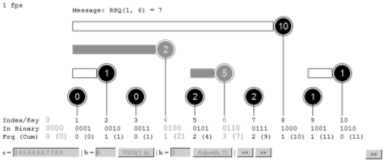
\includegraphics{img/t3}}
  \vspace{-5pt}
  \caption{树状数组的可视化}
  \label{fig:3}
\end{figure}
% \vspace{-10pt}

% !TEX root = ../../t.tex
\setlength{\belowcaptionskip}{-10pt}
\vspace{-7pt}
\begin{figure}[!htbp]
  \centering
  \frame{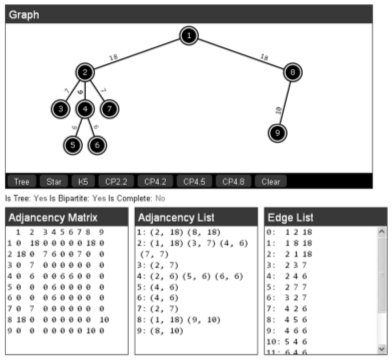
\includegraphics{img/t4}}
  \vspace{-5pt}
  \caption{图数据结构的可视化}
  \label{fig:4}
\end{figure}
% \vspace{-10pt}

\end{sectext}
\section{图}
\begin{sectext}
在网上有许多图的可视化。但是几乎所有的可视化都使用的是内嵌数据的方式,限制了使用方式。我们推测一方面由于难以为输入数据生成图的可视化,另一方面图的布局也是另一个难题。我们提供的可视化支持自定义绘图(如图\ref{fig:4})。自己绘图恰好可以消除我们对于布局算法的考虑。用户也可以添加、删除节点,在节点之间添加边,同时还可以指定方向和权值。用户调整可视化试图的同时,邻接矩阵、临界链表以及边链表也正确地自动更新。还有一个特点在于我们也会判断图的类别,包括树、二分图和完全图。
\end{sectext}
\section{图的遍历:深度优先搜索和广度优先搜索}
\begin{sectext}
在这个可视化中,用户可以像上述内容一样绘制图,然后运行任意一种经典的图遍历算法(DFS或者BFS)。许多关于图遍历的可视化都只实现了这些,但是鉴于这些DFS和BFS算法还包含有额外的关于图结构的信息,于是我们整合进新的特性。对于无向图上的DFS,还可以用Tarjan的算法来计算其强连通分量,如下面的静态图所示(如图\ref{fig:5})。在因特网上,现在也没有网站实现过DFS算法中这两个变量的可视化。对于无权图的BFS,还可以计算从起始点出发的所有最短路径。
% !TEX root = ../../t.tex
\setlength{\belowcaptionskip}{-10pt}
\vspace{-7pt}
\begin{figure}[!htbp]
  \centering
  \frame{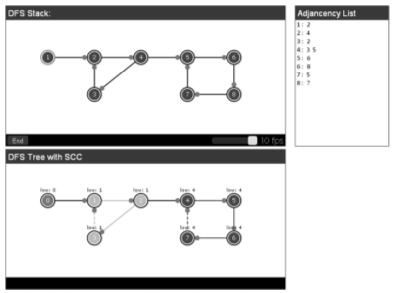
\includegraphics{img/t5}}
  \vspace{-5pt}
  \caption{遍历图的可视化(Tarjan强连通分量/DFS算法)}
  \label{fig:5}
\end{figure}
% \vspace{-10pt}

\end{sectext}
\section{最小生成树(MST):Prim算法和Kruskal算法}
\begin{sectext}
MST算法的可视化确实可以在网上找到,但是下面这个可视化的优势在于用户可以通过绘制图(同时与上述可视化有着相似的用户界面)来了解经典的Prim算法和Kruskal算法在图上的执行。我们还增加额外的功能,把所有边取负后就可以求得最大生成树(如图\ref{fig:6})。
% !TEX root = ../../t.tex
\setlength{\belowcaptionskip}{-1pt}
\vspace{-7pt}
\begin{figure}[!htbp]
  \centering
  \frame{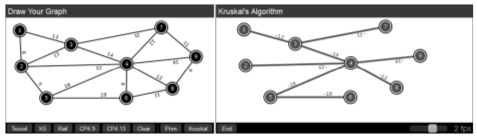
\includegraphics[width=440pt]{img/t6}}
  \vspace{-5pt}
  \caption{MST的可视化(Kruskal算法在用户输入数据的图上执行,其结果中边的权值全部取负)}
  \label{fig:6}
\end{figure}
% \vspace{-10pt}

\end{sectext}
\section{单源最短路径(SSSP):Dijkstra算法和Bellman Ford算法}
\begin{sectext}
SSSP算法的可视化在网上也有很多(特别是Dijkstra算法),但对于使用较少的Bellman Ford算法,其可视化却几乎没有。该算法可视化依然保持一致的用户界面,发挥同样的优势:学生可以自己绘制图。我们还提供SSSP的生成树,方便学生查看最短路径的信息。
% !TEX root = ../../t.tex
\setlength{\belowcaptionskip}{-10pt}
\vspace{-7pt}
\begin{figure}[!htbp]
  \centering
  \frame{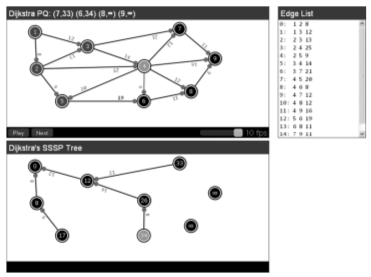
\includegraphics{img/t7}}
  \vspace{-5pt}
  \caption{SSSP的可视化(当源点为1时Dijkstra算法的执行)}
  \label{fig:7}
\end{figure}
% \vspace{-10pt}

\end{sectext}
\section{网络最大流:Edmond Karp算法}
\begin{sectext}
网上网络最大流算法的可视化非常少。我们的可视化(如图\ref{fig:8})有着同样风格的界面,与其他可视化一样也可以自定义图的结构。以后(第五节)我们还会增加不同网络流的模型和变形,加强可视化的效果。
% !TEX root = ../../t.tex
\setlength{\belowcaptionskip}{-1pt}
\vspace{-7pt}
\begin{figure}[!htbp]
  \centering
  \frame{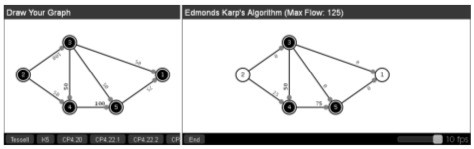
\includegraphics[width=440pt]{img/t8}}
  \vspace{-5pt}
  \caption{最大流的可视化(当源点为2汇点为1时Edmond Karp算法执行的结果)}
  \label{fig:8}
\end{figure}
% \vspace{-10pt}

\end{sectext}
\section{多边形算法:凸包判别、二维凸包}
\begin{sectext}
网上也有一些关于点集中寻找凸包的算法的可视化,但是大部分都是单一可视化。我们的可视化支持三种二维凸包算法:Graham的扫描算法(Graham,1972),如图\ref{fig:9}底部所示,Jarvis的卷包裹算法(Jarvis,1973)以及Andrew的单调链算法(Andrew,1979)。学生在使用这些功能的同时可以比较三种算法在同一个点集上的执行步骤。
% !TEX root = ../../t.tex
\setlength{\belowcaptionskip}{-10pt}
\vspace{-7pt}
\begin{figure}[!htbp]
  \centering
  \frame{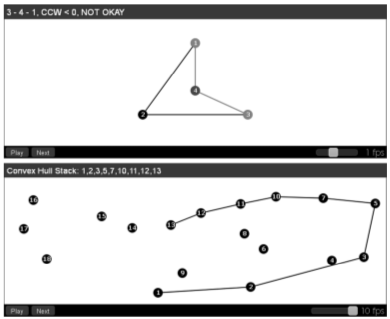
\includegraphics{img/t9}}
  \vspace{-5pt}
  \caption{算法执行过程,其中顶部为凸包判断,底部为Graham扫描算法}
  \label{fig:9}
\end{figure}
% \vspace{-10pt}

另外,对于多边形还有其他许多操作,例如判断任意多边形是凸多边形还是凹多边形(如图\ref{fig:9}顶部)、计算其面积和周长、判断点是否在给定凸多边形或者凹多边形的内部、用直线裁剪多边形。其中一些操作已经在可视化系统中实现,而剩余其他的一些操作将在以后扩展(第五节)。
\end{sectext}

% !TEX root = ../../t.tex
\chapter{学生反馈}
\begin{sectext}
新加坡国立大学第二学期中(2012年1--2月),在第三节中介绍的算法可视化首次用于两种模式:
\begin{itemlist}
\item CS3233——高级编程(24名学生),任课老师为第一位作者。使用到的可视化包括:位掩码、位表示、DFS、BFS、MST、SSSP、最大流和多边形凸包。

\item CS2020——数据结构和算法速成(42名学生),任课老师为第一位作者的同事,使用到的可视化包括:堆、位表示、DFS、BFS、MST、SSSP。
\end{itemlist}

我们对两个班的学生使用以下调研来测量这些可视化带来的主观效果。调研于2012年3月展开,两个班的学生都各自看过上述列举的可视化。其中第一位作者所带CS3233课程的班上所有24名(100\%)学生都表示广泛地使用过。而参加CS2020课程的学生中只有7名(16.7\%)学生表示没有经常使用。我们把这两组学生的结果分成下面的两列,可以看出整体上两组学生的反馈非常相近。
\end{sectext}
\section{多项选择题(MCQ)}
\begin{sectext}
% !TEX root = ../../t.tex
\begin{center}
\setstretch{1.35}
\vspace{-20pt}
\begin{longtable}{p{5cm} p{4cm} p{4cm}}
\caption{MCQ结果}
\label{tab:2} \\

\hline \multicolumn{1}{l}{多项选择题} & \multicolumn{1}{l}{CS3233(24名受访者)} & \multicolumn{1}{c}{CS2020(7名受访者)} \\ \hline
\endfirsthead

\multicolumn{3}{r}%
{接表 \ref{tab:2}} \\
\hline \multicolumn{1}{l}{多项选择题} & \multicolumn{1}{l}{CS3233(24名受访者)} & \multicolumn{1}{c}{CS2020(7名受访者)} \\ \hline
\endhead

\hline \multicolumn{3}{r}{待续}
\endfoot

\hline
\endlastfoot

1、算法可视化是否帮助你更好地理解算法? & 有 (13/54.1\%)\par 没有 (0/0.0\%)\par 一般 (11/45.8\%) & 有 (5/71.4\%)\par 没有 (0/0.0\%)\par 一般 (2/28.5\%) \\
2、你什么时候使用算法可视化?(多选) & 课上 (8/33.3\%)\par 课后 (4/16.6\%)\par 考试前 (14/58.3\%)\par 其他 (6/25.0\%) & 课上 (1/14.2\%)\par 课后 (0/0.0\%)\par 考试前 (5/71.4\%)\par 其他 (3/42.9\%) \\
3、你如何访问算法可视化的网站?(多选) & 台式电脑 (14/58.3\%)\par 笔记本 (14/58.3\%)\par 平板电脑 (3/12.5\%)\par 智能手机 (5/20.8\%) & 台式电脑 (4/57.1\%)\par 笔记本 (6/85.7\%)\par 平板电脑 (0/0.0\%)\par 智能手机 (1/14.2\%)\\

\end{longtable}
\end{center}
\vspace{-42pt}

下面是几个对于问题1回答理由的节选:

有:对于视觉来说很直观;有助于解释概念;可以自己输入不同的数据;有助于一开始了解算法的执行;以前一直是自己手画这些例子。

一般:已经通过授课、书本、源代码了解过算法;之前已经掌握;更希望通过分析证明而不是可视化的方式来展示算法的执行;可视化过程中(这是用于上课的版本)出现了错误,影响算法的理解。

值得一提的是在32一个受访者中没有一人选择``没有,算法可视化没有让我对算法理解地更深''。因此这些可视化可以看作是一种教学辅助工具,极大帮助了一部分学生,同时不会对其他学生产生不好的影响。

从第二个MCQ中我们可以看出学生在课堂上能够参与讨论。而最常见的使用方式则是在测试、测验前使用。这说明可视化主要用于自学和复习。

从第三个MCQ中我们可以看出一些学生使用智能手机或者平板电脑访问可视化网站。虽然使用人数上还是比较少,但是并不是每个人都有这些设备,我们还是相信这种情况在未来会有所改善。
\end{sectext}
\section{开放式问答题}
\begin{sectext}
我们也为同学们准备了一些开放式问答题。首先请学生列出这些算法可视化的好处和坏处。一些有代表性的反馈列在表\ref{tab:3}中。
% !TEX root = ../../t.tex
\begin{center}
\setstretch{1.35}
\vspace{-20pt}
\begin{longtable}{p{7cm} p{7cm}}
\caption{算法可视化的效果}
\label{tab:3} \\

\hline \multicolumn{1}{l}{积极方面} & \multicolumn{1}{l}{消极方面} \\ \hline
\endfirsthead

\multicolumn{2}{r}%
{接表 \ref{tab:3}} \\
\hline \multicolumn{1}{l}{积极方面} & \multicolumn{1}{l}{消极方面} \\ \hline
\endhead

\hline \multicolumn{2}{r}{待续}
\endfoot

\hline
\endlastfoot

算法可视化能直接给出正确答案(在修复程序错误后)。 & 算法可视化的程序错误在早期测试使用中会影响理解。\\
简介的用户界面,易于使用。 & 一些功能对用户还不够友好(还缺少合适的教程文档)。\\
用户能使用自己的例子:输入具体数据、绘制图和多边形。 & 在CS3233教学中需要的算法可视化不仅仅是上述的九种。\\
有助于更好地理解算法。 & 有了算法可视化可能导致学生不主动练习。\\
比徒手模拟更快。 & 可视化的每个步骤最好配上算法的(伪)代码。\\
\end{longtable}
\end{center}

\vspace{-42pt}


接着,我们还询问学生对于这样一个统一界面网站的看法,网站中不仅仅有上述列举的九种可视化,在将来还会有更多。一些节选回复如下:

好:不仅有利于这门课程(CS3233)也对NUS其他算法课程或其他大学有帮助。

好:统一的界面非常好。学生通常会像可视化那样在心里或者纸上模拟算法。

一般:这是个好主意。但是要是没有这样的网站问题也不大。

不好:我个人更喜欢自己动手模拟算法,这并不困难,而且也帮助我更好地记忆算法。但我相信肯定有其他人会喜欢这种工具。
\end{sectext}

% !TEX root = ../../t.tex
\chapter{初步结论、未来展望、致谢}
\begin{sectext}
在本论文中,我们展示了一共九个算法可视化,这些可视化都有一致的风格、界面,由HTML5技术和Javascript编写支撑,同时还支持用户交互。31名学生中一半以上表示有助于学习,而其余则表示效果一般。

这个可视化项目还是一个正在不断完善的项目。现在,可以访问 \url{www.comp.nus.edu.sg/~stevenha/visualization} 查看该项目。这个URL地址可能以后会有所变化,但下面的一些关键词有助于重新在网上找到该项目:``算法''、``可视化''、``高级编程''、``SoC''、``NUS''以及作者的名字。

之后,我们有以下的计划:
\begin{itemlist}

\item 强化现有可视化的功能:增加最小树形图(树状)的朱刘、Edmonds算法(朱永津和刘振宏,1965;Edmonds,1967)、各种网络流模型和变形(例如:二分匹配、最小费用流等)和一些多边形上的算法。

\item 增加更多经典算法,完善算法可视化库,现在已经实现了算法包括:DAG上的算法(例如:最短路、最长路、路的数量)、树(例如:最近公共祖先等)。

\item 增加更多网上没有的非经典算法的可视化,例如线段树、Edmonds的最大匹配算法(Edmonds,1965),Hopcroft Karp的二分匹配算法(Hopcroft Karp,1973),后缀数组以及后缀树表示(Manber和Myers,1991)等。

\item 优化用户界面,使可视化更加对用户更加友好(尤其是在可视化的同时添加源代码高亮,以及添加``后退''功能)。

\item 提供更多教学使用场景,例如弹出对话框,测试下一步应该是怎样执行。

\item 扩展可视化系统,让其他开发者使用我们的API
\end{itemlist}

我们希望该可视化项目能够在世界各地的大学、计算机院系中得到使用。

本论文所有的作者非常感谢新加坡国立大学发展教学与学习中心(CDTL,NUS)提供该可视化项目的启动资金。
\end{sectext}

\bibliography{}
\begin{chatext}
{
\leftskip 2em
\parindent -2em

Andrew, A.M. (1979). Another efficient algorithm for convex hulls in two dimensions. \textit{Information Processing Letters}, 9, 216–219.

Chu, Y.J., Liu, T.H. (1965). On the shortest arborescence of a directed graph. \textit{Science Sinica}, 14, 1396–1400.

Edmonds, J. (1965). Paths, trees, and flowers. \textit{Canadian Journal of Mathematics}, 17, 449–467.

Edmonds, J. (1967). Optimum Branchings, \textit{Journal of Research of the National Bureau of Standards}, 71B, 233–240.

Edmonds, J., Karp, R.M. (1972). Theoretical improvements in algorithmic efficiency for network flow problems. \textit{Journal of the ACM}, 19(2), 248–264.

Fenwick, P.M. (1994). A new data structure for cumulative frequency tables. \textit{Software: Practice and Experience}, 24(3), 327–336.

Forišek. M. (2009). \textit{IOI Syllabus}. \url{http://people.ksp.sk/∼misof/ioi-syllabus/}. Last accessed 11 April 2012.

Graham, R.L. (1972). An efficient algorithm for determining the convex hull of a finite planar set. \textit{Information Processing Letters}, 1, 132–133.

Halim, S., Halim, F. (2011). \textit{Competitive Programming 2: This increases the lower bound of programming contests. Again.} \url{http://www.lulu.com}.

Hopcroft, J.E., Karp, R.M. (1973). An n 5/2 algorithm for maximum matchings in bipartite graphs. \textit{SIAM Journal on Computing}, 2(4), 225–231.

Jarvis, R.A. (1973). On the identification of the convex hull of a finite set of points in the plane. \textit{Information Processing Letters}, 2, 18–21.

Manber, U., Myers, G. (1991). Suffix arrays: a new method for on-line string searches. \textit{SIAM Journal on Computing}, 22(5), 935–948.

Tarjan, R.E. (1972). Depth-first search and linear graph algorithms. \textit{SIAM Journal on Computing}, 1(2), 146–160.

}
\end{chatext}
